\documentclass{article}



\usepackage{arxiv}

\usepackage[utf8]{inputenc} % allow utf-8 input
\usepackage[T1]{fontenc}    % use 8-bit T1 fonts
\usepackage{amsmath,amssymb,amsfonts,float,graphicx,bm,psfrag,amsmath,amsthm}
\usepackage{algorithm, algorithmic,CJK,color,colortbl,geometry,url,hyperref}
\usepackage{graphicx,cite,bm,psfrag,amsmath}
\usepackage{enumerate}
\usepackage{subfigure}
\usepackage{booktabs}         


\title{Project Report}

%\date{September 9, 1985}	% Here you can change the date presented in the paper title
%\date{} 					% Or removing it

\author{Mingqi Yuan}

% Uncomment to remove the date
%\date{}

% Uncomment to override  the `A preprint' in the header
%\renewcommand{\headeright}{Technical Report}
%\renewcommand{\undertitle}{Technical Report}
\renewcommand{\undertitle}{}
\renewcommand{\headeright}{}
\renewcommand{\shorttitle}{}

%%% Add PDF metadata to help others organize their library
%%% Once the PDF is generated, you can check the metadata with
%%% $ pdfinfo template.pdf
\hypersetup{
pdftitle={A template for the arxiv style},
pdfsubject={q-bio.NC, q-bio.QM},
pdfauthor={David S.~Hippocampus, Elias D.~Striatum},
pdfkeywords={First keyword, Second keyword, More},
}
\date{}

\begin{document}
\maketitle

\begin{abstract}
	Python implementation of the UniNet for iris recognition which is proposed in \cite{zhao2017towards}.
\end{abstract}


% keywords can be removed
\keywords{Iris recognition \and Python \and Pytorch}

\section{Brief summary}
Dear Professor, thanks again for the valuable opportunity! This project is challenging and interesting, and I learn a lot from that. Because I have never been involved in projects about the iris recognition before, so it takes me some time to learn the corresponding theory. Moreover, because the TensorFlow can not realize the special gradients of ETL loss, I have to learn the PyTorch temporarily and rewrite the whole project. No matter whether I can pass the test, I sincerely hope that you can help me point out the shortcomings. And I'd appreciate it much if you can provide your codes for me. Thank you very much!

I have uploaded the project (contains no training data) to the GitHub, and you can check the details in the following url.

\textcolor{blue}{\url{https://github.com/Mingqi-Yuan/UniNet}}

\section{Project structure}
This project is organized as follows:
\begin{itemize}
	\item \textbf{dataset}: contains the training data, validation data and test data. 
	\item \textbf{reference}: contains the reference materials.
	\item \textbf{report}: contains the LaTex files of the project report.
	\item \textbf{snapshots}: for saving model weights.
	\item \textbf{static}: contains the pretrained model (MaskNet) and so on.
	\item \textbf{data.py}: for constructing the data generator.
	\item \textbf{eval.py}: for calculating TAR, FAR, EER.
	\item \textbf{loss.py}: the implementation of the \textit{Extended Triplet Loss}.
	\item \textbf{mask.py}: for predicting masks for all the images in dataset using the pretrained MaskNet.
	\item \textbf{match.py}: functions for the iris matching (e.g. Hanmming distance).
	\item \textbf{model.py}: model class of the UniNet.
	\item \textbf{network.py}: the implementation of the FeatNet and the MaskNet.
	\item \textbf{train.py}: training file.
\end{itemize}

\section{class ETLoss}
In this section, the implementation of the \textit{Extended Triplet Loss} are elaborated in detail. The ETLoss class contains four major functions:

\begin{enumerate}[1)]
	\item \textbf{shiftbits(self, fa, noshifts)} This function is used to calculate the shifted features.
	\item \textbf{fd(self, f1, f2, mask1, mask2)} This function is used to calculate the \textit{Fractional Distance} between two features.
	\begin{figure}[h]
		\centering
		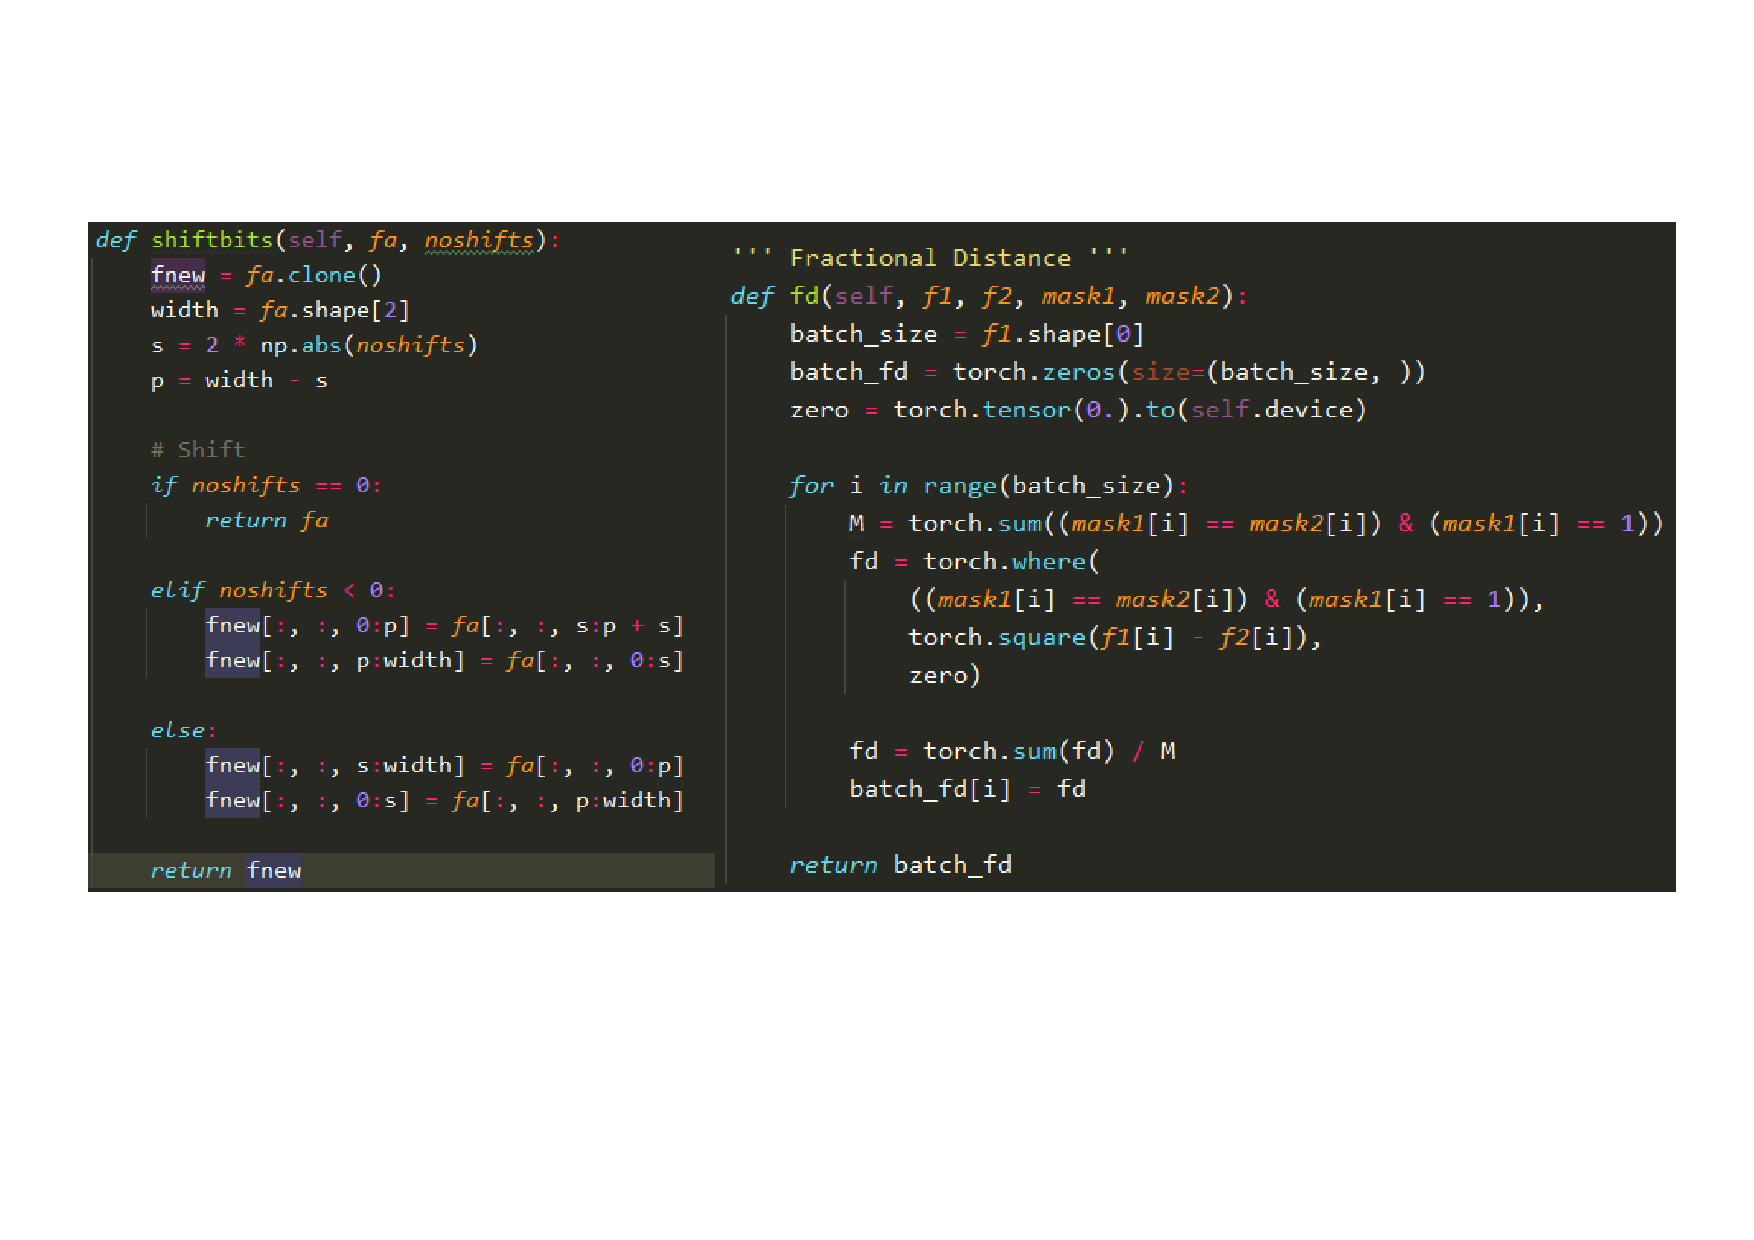
\includegraphics[width=0.9\linewidth]{figs/sbfd.pdf}
	\end{figure}

	\item \textbf{mmsd(self, f1, f2, mask1, mask2)} This function is used to calculate the \textit{Minimum Shifted and Masked Distance}.
	\item \textbf{foward(self, fp, fa, fn, fp\_mask, fa\_mask, fn\_mask)} This function is used to calculate the final loss.
	
	\begin{figure}[h]
		\centering
		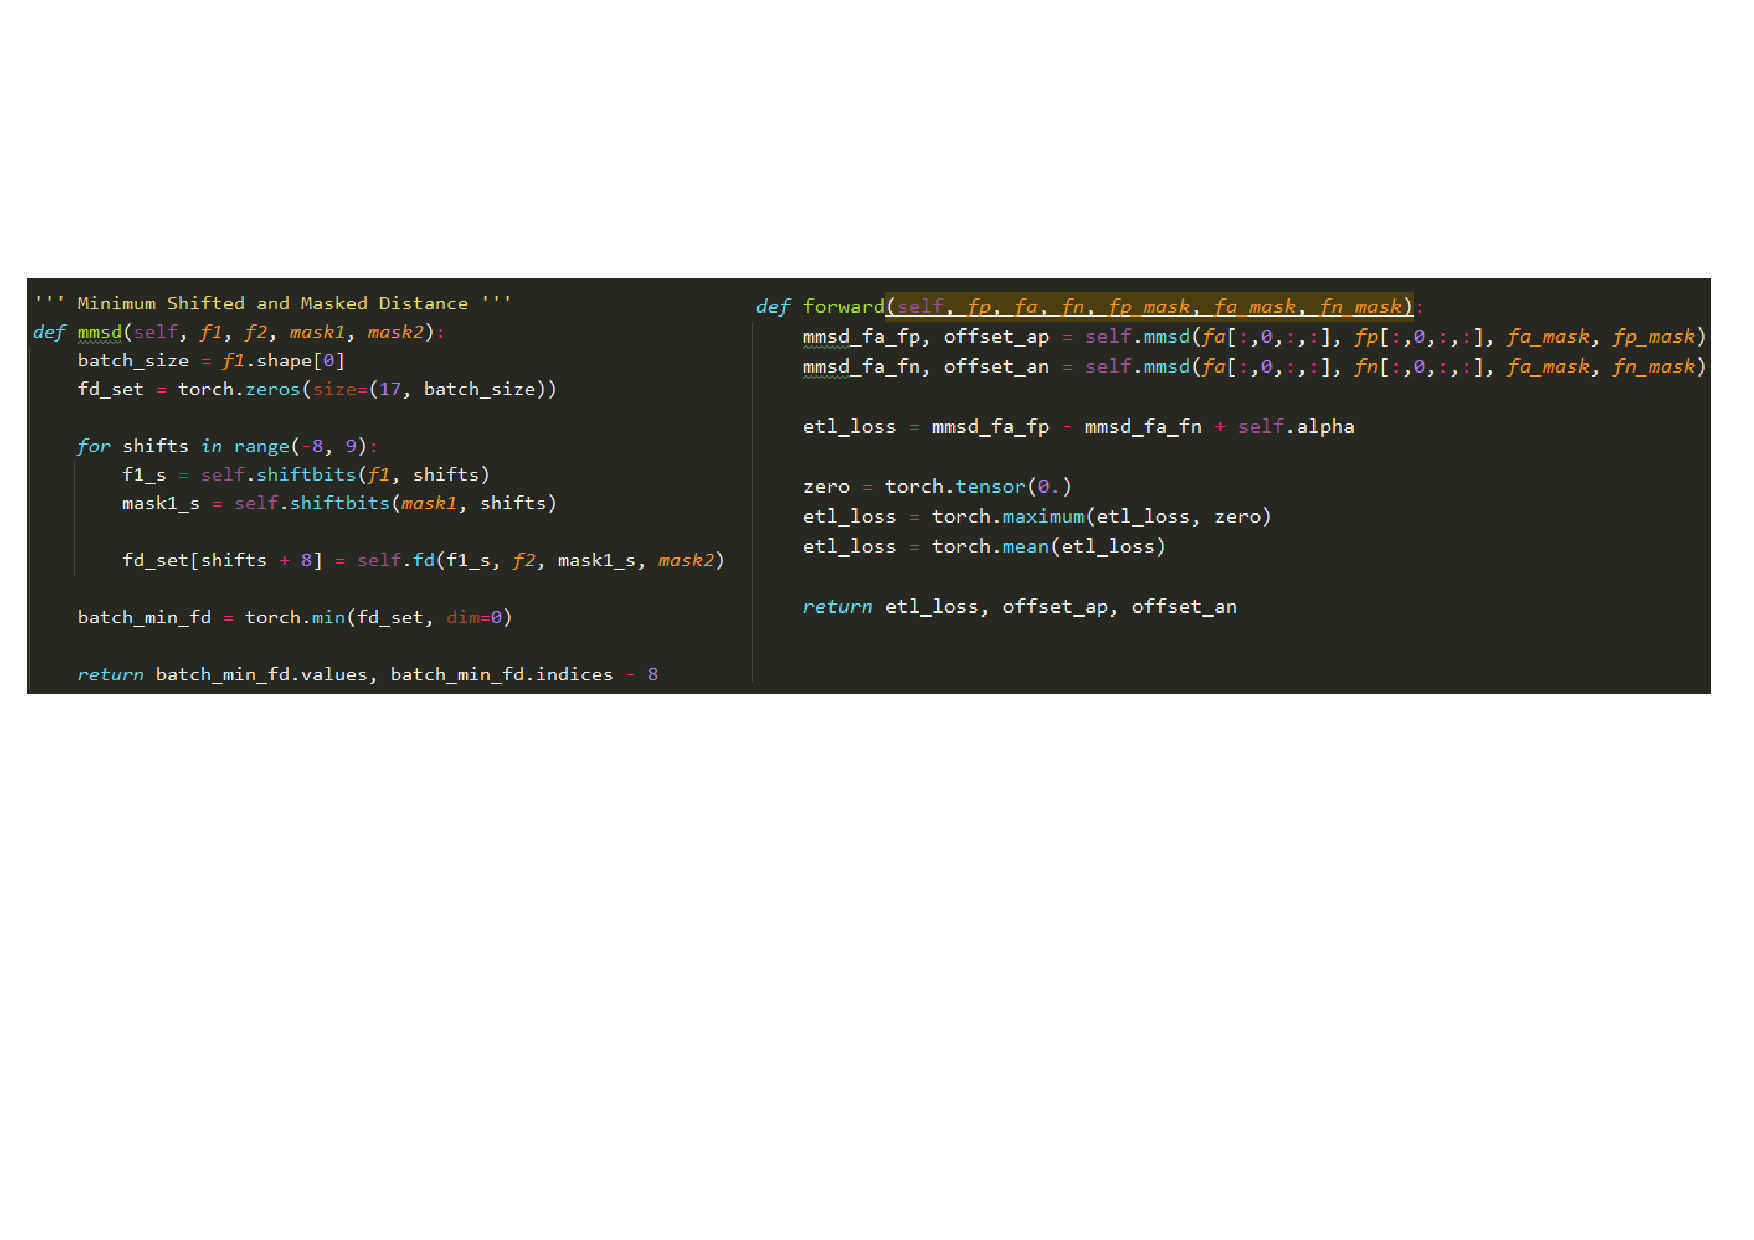
\includegraphics[width=0.9\linewidth]{figs/mmsdfor.pdf}
	\end{figure}
\end{enumerate}

\section{Gradients of $\frac{\partial ETL}{\partial\mathbf{f}^{P}[x,y]},\frac{\partial ETL}{\partial\mathbf{f}^{A}[x,y]},\frac{\partial ETL}{\partial\mathbf{f}^{N}[x,y]}$}

The ETL takes the shifted feature to get the final loss, which has special gradients definitions. When applying the back propagation, the AutoGrad tool of PyTorch will automatically calculate all the requisite gradients. But such gradients is different from the original definitions, which are needed to be replaced. So the following codes are leveraged to address the problem.

\begin{itemize}
	\item etl\_loss, b\_AP, b\_AN = self.etl\_loss.forward(fp, fa, fn, img\_ps\_mask, img\_as\_mask, img\_ns\_mask)	\textcolor{red}{\#} get the etl loss, $b_{AP}, b_{AN}$ for the batch features.
	\item fp.retain\_grad() \textcolor{red}{\#} obtain the gradients of $f^{P}$.
	\item fa.retain\_grad() \textcolor{red}{\#} obtain the gradients of $f^{A}$.
	\item fn.retain\_grad() \textcolor{red}{\#} obtain the gradients of $f^{N}$.
	\item etl\_loss.backward()
	\item grad\_etl2fp, grad\_etl2fa, grad\_etl2fn = self.get\_grad(etl\_loss, fp, fa, fn, img\_ps\_mask, img\_as\_mask, img\_ns\_mask, b\_AP, b\_AN) \textcolor{red}{\#} get new gradients.
	\item fp.grad.data = grad\_etl2fp.data \textcolor{red}{\#} replace the old gradients.
	\item fa.grad.data = grad\_etl2fa.data
	\item fn.grad.data = grad\_etl2fn.data 
	\item self.optimizer.step() \textcolor{red}{\#} apply the BP process.
\end{itemize}

The \textbf{self.get\_grad()} can be found in the \textbf{model.py}, which is used to calculate the gradients for the ETL.

\section{Triplet input}
The data generator defined in the \text{data.py} follows the selection method of the \textit{facenet} repository in GitHub:

\textcolor{blue}{\url{https://github.com/davidsandberg/facenet/blob/master/src/train_tripletloss.py}}

The only difference is the embedding form, which is a vector in facenet and a feature matrix in UniNet.

\section{Training and evaluation}
In view of the short time and limited devices (I have two RTX2080Ti GPU, each one only have 11Gb video memory.), so I have to use a part of the whole dataset to conduct the training, and the triplet input for each epoch is not comprehensive enough. The following results are based on the iris images of the former 50 people, which only aims to test the correctness the program. And the ROC is obtained with the randomly-selected pairs in validation data.

\begin{table}[h]
	\centering\caption{Part of the training parameters}
	\begin{tabular}{cccc}
		\toprule[1.5pt]
		batch size & people number for per epoch & images number of per person & alpha \\ \midrule[1.5pt]
		20         & 25                          & 40                          & 0.2 \\ \bottomrule[1.5pt]
	\end{tabular}
\end{table}
\begin{figure*}[h]
	\centering
	\subfigure[Training loss]{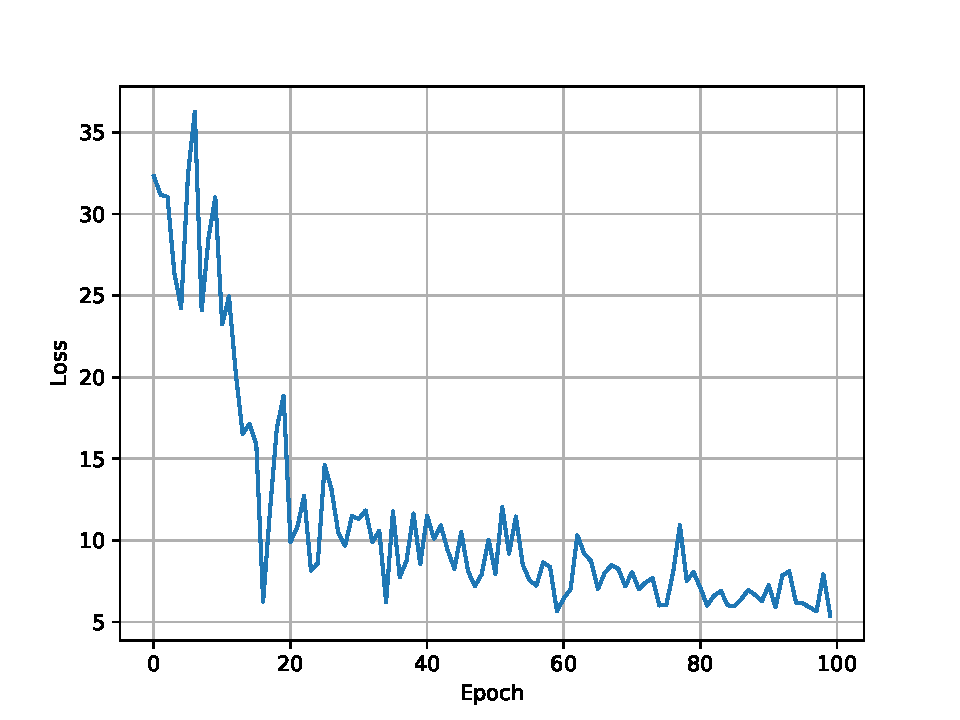
\includegraphics[width=0.45\linewidth]{figs/loss.pdf}}
	\subfigure[ROC curve]{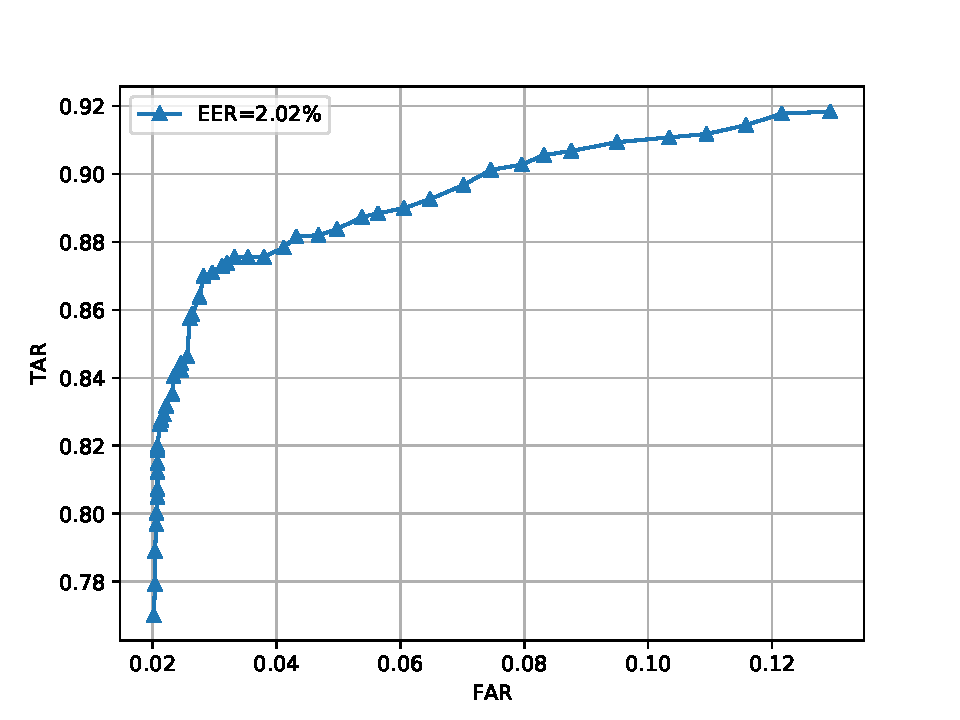
\includegraphics[width=0.45\linewidth]{figs/roc.pdf}}	
	\caption{Simulation results}
\end{figure*}


\bibliographystyle{unsrtnat}
\bibliography{reference}

\end{document}
